\section{Tarea periódicas y continuas}
\textbf{PLC y estructuras para planta 4 estanques.Tareas para tiempo real en PLC, configuración de tareas (no) periódicas,  variables locales y globales, efectos de scan fijo y variable.}
\subsection{Tareas}
En \textit{Studio 5000} las tareas están definidas como periodicas, continuas o eventos. Esto crea una jerarquía de ejecución donde es de suma importancia la elección de un tiempo de muestreo lo suficientemente rápido para asegurar que los algoritmos de co trol capturen la dinámica del sistema sin perjudicar la ejecuciónde tareas continuas.

\begin{figure}[H]
  \begin{center}
    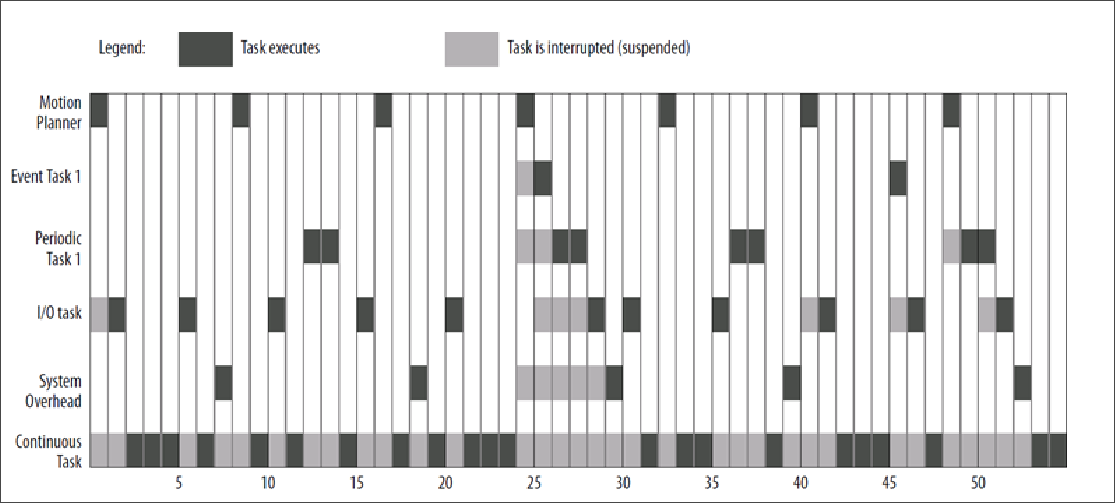
\includegraphics[width=0.8\textwidth]{figures/tareas.png}
  \end{center}
  \caption{Tareas (tomado de \textbf{rockwellGeneralInstructions})\cite{rockwellGeneralInstructions}}\label{fig:tareas}
\end{figure}

Las tareas periodicas comprenden todo lo que es algoritmos de calculo y muestreo deterministico, las tareas continuas por otro lado se encargan  de las alarmas y advertencias, finalmente las tareas eventos son tareas de muy alta prioridad que interrumpen el proceso cuando lo requieran. 

\subsection{ScanTime}
Por \textit{ScanTime} se define el tiempo total que le demora al PLC en completar una vuelta de las tareas continuas considerando todas las interrupciones causadas por tareas periodicas en medio. Por esto es imperativo escoger un tiempo de meustreo adecuado, normalmente este elige tomando en consideración que sea al menos 5 veces más rápido que la constante de tiempo más rápida del sistema. Este criterio deber ser contrastado con la necesidad de no aumentar el \textit{ScanTime} innecesariamente, esto porque entre más pequeño es el timepo de muestreo, más veces se ejecutará la tarea periodica en un tiempo determinado, quitando tiempo de ejecución a las tareas continuas, generando que el \textit{ScanTime} aumente.

Esto puede generar problemas de comunicaciónn con la HMI, lag entre los datos desplegados o alarmas.

\subsection{Tipos de variables}

Las variables o tags en \textit{Studio 5000} tienen dos características principales, su \textit{scope} y su tipo. Por \textit{scope} se entiende el alcance que tiene una variable y qué programas tienen acceso a distintas variables. En la arquitectura Logix de Rockwell Automation, este alcance se divide estrictamente en dos niveles fundamentales:

\begin{itemize}
    \item \textbf{Controller Scope (Alcance Global):} Las variables declaradas bajo el contenedor \textit{Controller Tags} poseen un alcance global dentro de todo el procesador. Esto implica que cualquier rutina, sin importar el programa ejecutor al que pertenezca, puede leer o escribir sobre ellas. Son obligatoriamente de \textit{Controller Scope} las variables de acoplamiento físico (como las entradas y salidas analógicas/digitales mapeadas a los módulos de hardware), así como aquellas que sirven de puente de datos mediante el servidor OPC UA (\textit{FactoryTalk Gateway}) hacia elementos externos como la interfaz SCADA/HMI o los scripts de sintonía en MATLAB (por ejemplo, el tag global \textit{Switch\_Valores\_Iniciales} o las señales \textit{LIT\_01.PV} y \textit{FIC\_01.SP}).
    \item \textbf{Program Scope (Alcance Local):} Las variables declaradas dentro de un programa específico (\textit{Program Tags}) están encapsuladas y son invisibles para rutinas fuera de dicho contenedor. Este diseño modular previene la corrupción inadvertida de memoria. En el contexto de la planta de 4 estanques, es una buena práctica de ingeniería clasificar como locales las variables matemáticas auxiliares y los estados transitorios asociados a los algoritmos avanzados de control discreto (tales como los errores previos del lazo $e(k-1)$, acumuladores de la acción integral, o buffers de retraso del predictor de Smith), dado que su existencia solo es relevante para el cálculo interno de esa rutina particular.
\end{itemize}

Por otro lado, el \textit{tipo} define la naturaleza de los datos y la estructura en memoria que el procesador asignará para su almacenamiento y manipulación. Las variables se catalogan en tipos fundamentales o estructuras complejas:

\subsubsection{Tipos de Datos Principales }
Constituyen los bloques de memoria primitivos sobre los cuales opera la CPU del controlador:
\begin{itemize}
    \item \textbf{BOOL (Booleano):} Ocupa un bit de información. Representa estados lógicos binarios (0 o 1). Se utiliza para mandos y enclavamientos de seguridad operativos en el código, como la habilitación del lazo en modo automático/manual o alarmas binarias de procesos discretos.
    \item \textbf{DINT (Double Integer):} Entero de doble precisión con signo que ocupa 32 bits en memoria. Es ideal para contadores, selectores indexados de menús de navegación o almacenamiento de palabras de estado (\textit{Status Word}) donde cada bit individual codifica condicionales operacionales lógicas direccionables en base a enmascaramientos binarios.
    \item \textbf{REAL (Floating Point):} Ocupa de igual forma 32 bits de memoria, pero distribuidos bajo la norma de coma flotante IEEE 754. Es el tipo de dato mandatorio para variables continuas analógicas del proceso. En la planta de control, sensores de nivel (\textit{LIT}) y transmisores de flujo (\textit{FIT}) deben ser obligatoriamente de tipo \textit{REAL} para preservar la precisión decimal indispensable en el cómputo de la acción integral y el filtro derivativo en el Texto Estructurado; el uso erróneo de tipos enteros generaría un truncamiento numérico que inutilizaría las dinámicas transitorias del control digital.
\end{itemize}

\subsubsection{Estructuras de Datos y Tipos de Parámetros}
Adicionalmente, para simplificar el flujo y la organización de la base de datos de tags, \textit{Studio 5000} permite emplear tipos de datos estructurados complejos. Un claro ejemplo de esto se observa al programar instrucciones personalizadas Add-On (\textit{AOI}), donde las variables internas pueden clasificarse bajo el estándar de paso de parámetros:
\begin{itemize}
    \item \textbf{Input Parameters:} Variables analógicas o digitales de solo lectura que el bloque de control requiere desde el proceso en cada periodo de muestreo $T_s$ (ej: la variable de proceso actualizada $PV$ o las referencias de setpoint $SP$).
    \item \textbf{Output Parameters:} Variables calculadas por el algoritmo que se disponibilizan de solo escritura hacia la planta o el entorno de visualización (ej: la variable manipulada final calculada $CV$ dirigida al variador de frecuencia de la bomba).
    \item \textbf{InOut Parameters (Paso por referencia):} Estructuras de datos complejas que se transfieren mediante punteros de memoria directos. Son fundamentales para pasar matrices de coeficientes lógicos en estimadores en tiempo real o bases de datos complejas de alarmas compartidas dinámicamente, evitando duplicar el uso de la memoria física del procesador ControlLogix.
\end{itemize}
